% Eye as a Camera in XR. IEEE ICCE 2027 (Las Vegas), IEEE conference template.
% Draft for co-authors. Red [TODO] marks are open; [RF] marks are for Rich Fletcher.
\documentclass[conference]{IEEEtran}
\IEEEoverridecommandlockouts
\usepackage{cite}
\usepackage{amsmath,amssymb}
\usepackage{graphicx}
\usepackage{booktabs}
\usepackage{xcolor}
\usepackage{url}
\usepackage[hidelinks]{hyperref}
\graphicspath{{figures/}}

\newcommand{\todo}[1]{\textcolor{red}{[TODO: #1]}}
\newcommand{\rf}[1]{\textcolor{blue}{[RF: #1]}}
\newcommand{\dprime}{d^{\prime}}

\begin{document}

\title{Eye as a Camera in XR: Reading Images, Colours and Eye Strain from a Consumer EEG Headband and a Consumer VR Headset}

\author{
\IEEEauthorblockN{Alexander Vicol\IEEEauthorrefmark{1}, Mikey Herreraviyella\IEEEauthorrefmark{1}, Minu Adefris\IEEEauthorrefmark{1}, Khalil Chaghouri\IEEEauthorrefmark{1},\\
Ali Sher\IEEEauthorrefmark{1}, Richard R. Fletcher\IEEEauthorrefmark{2}, and Steve Mann\IEEEauthorrefmark{1}}
\IEEEauthorblockA{\IEEEauthorrefmark{1}University of Toronto and MannLab Canada, Toronto, Canada\\
\IEEEauthorrefmark{2}Mobile Technology Group, Massachusetts Institute of Technology, Cambridge, USA\\
vicola.lexo@gmail.com}
% TODO: confirm each author's affiliation and email, and the order, with everyone named here
}

\maketitle

\begin{abstract}
Mann showed in 2019 that the eye can be used as a camera: a square flickers at one position after another, the subject follows it, and the steady-state visual evoked potential (SSVEP) says how bright each position was. We move the method onto hardware a community health worker could carry: a Muse 2 headband with one cup electrode added over the visual cortex, and a Meta Quest 3S running the stimulus in its browser. We read a legible word in 18 minutes ($r = 0.91$ against time-shifted nulls of 0.23), eight colours as three calibrated colour planes (24 of 32 cells, reproduced over three sittings), and an acuity optotype drawn at random and sealed before the scan, named correctly from the EEG alone. The same recording gives an objective eye-strain reading: blinks stop while a cell flickers and burst when it goes dark, and the blink rate doubled between two sittings of one evening. We frame the result as a literacy-free visual screener in the tradition of low-cost mobile health tools, with a prompt to rest the eyes as its first intervention. All results are from one subject.
\end{abstract}

\begin{IEEEkeywords}
SSVEP; EEG; extended reality; consumer electronics; brain-computer interface; mobile health; visual screening; eye strain; just-in-time adaptive intervention; wearable computing.
\end{IEEEkeywords}

\section{Introduction}

A camera needs a lens, a sensor and a readout. The eye has the first two; Mann's ``eye as a camera'' \cite{mann2019eye, mann2019wearsys} supplied the third. A square flickers at a fixed rate, the subject looks at it, and the visual cortex answers with an SSVEP whose strength follows the light the square puts into the fovea \cite{norcia2015ssvep, vialatte2010ssvep}. Scan the square across an image and the sequence of strengths is the image. The 2019 paper read ``NO CAMERAS'' and a portrait with a laboratory amplifier and 85 minutes of scanning.

This paper asks what the method can do on hardware that costs less than a phone and needs no technician: a Muse 2 headband (about \$250) with one cup electrode through its auxiliary input, a Meta Quest 3S (about \$300) running the stimulus as a web page, and a laptop. Our interest comes from the mobile health tradition of low-cost sensing in the hands of community health workers \cite{fletcher2010wearable, fletcher2017child, anand2018pulmonary}. A visual screen read from the EEG asks the subject to name no letter and press no button; they look at a dot. The same recording carries what the mobile health literature has long wanted from wearables, an objective reading of the subject's state \cite{fletcher2010icalm, fletcher2014mental}, here the eye strain that flicker produces.

We contribute: the first SSVEP imaging on a consumer VR headset with a consumer headband; colour by three calibrated planes; a sealed, objective acuity read-out; eye strain from the same recording; and the field engineering that made the method survive outside a laboratory, with a synthetic subject as regression test.

\section{Background}

The SSVEP is largest over the occipital midline (Oz) and strongest for stimuli in the central field \cite{norcia2015ssvep}, which is what makes a single flickering patch under the gaze one pixel per position \cite{mann2019eye}. SSVEP interfaces in head-mounted displays are established \cite{armengol2018sublime}; imaging on one, and on the Quest family, is not.

\textbf{Metaveillography of the eye.} The eye-as-camera idea grew out of a longer programme on seeing sight itself. Mann photographed a camera's capacity to see with a light that brightens when the camera sees it, the sightfield, a time-reversed lightfield captured by long exposure \cite{mann2014sightfield}, and named the sensing of sensors and of their capacity to sense metaveillance \cite{mann2016metaveillance}; the photographs are metaveillographs, the measurements metaveillogrammetry \cite{mann2021drones}. Janzen and Mann turned the method on the human eye, measuring how far its sensing extends through space as a biological veillance flux \cite{janzen2014veillance, janzen2015veillametrics}, and time-integrating that flux on objects as a veillogram, a sensory map of what a person's gaze has actually taken in \cite{janzen2018painting}. The 2019 paper let the brain report instead of the subject: a brain-modulated LED carried through the visual field by a plotter, its brightness set by the SSVEP from a Muse headband, photographed over a long exposure into a metaveillograph of the eye's own receptive field \cite{mann2019eye, mann2019wearsys}. The same group then mapped the visual field into a ``vidmap'' \cite{garcia2020painting} and read acuity from the SSVEP in a healthcare IoT volume \cite{garcia2021acuity}. Two findings there are the health claims this paper builds on. The veillance field narrows when the observer fixates and ignores the flicker and widens when they track it, so it measures attention and not only optics, which the 2019 paper proposed as a biomarker for attention problems in ADHD and ageing, ``the vision test of the future'' \cite{mann2019eye}. And the read-out is evidence rather than testimony: nobody has to say what they see. The sweep VEP reads acuity without a verbal response \cite{norcia1985sweep}; our optotype read-out is a coarse, gaze-scanned relative of it. Chromatic VEPs differ by colour axis and temporal frequency \cite{rabin1994chromatic}, which is why our colour planes are calibrated separately. The Muse headband is validated for event-related potentials \cite{krigolson2017muse} but has no electrode near Oz; the added cup is what makes imaging possible (cup alone $r = 0.92$, ear electrodes alone 0.36). A VR headset over the Muse improves the contact rather than degrading it \cite{mann2026float}.

Fletcher's group has built a decade of diagnostics around sensors a phone already has, for workers who are not specialists: pulmonary screening from cough and lung sounds \cite{chamberlain2016asthma, infante2017cough, anand2018pulmonary}, child health tools \cite{fletcher2017child}, printed diagnostics read by the camera \cite{fletcher2016printed}, thermal imaging with deep learning \cite{fletcher2021thermal, byun2021thermal}, blood pressure from photoplethysmography \cite{elgendi2019ppg}, and hand-vein patient identification \cite{fletcher2014vein}. Vision screening is a gap in that list: the Snellen chart and the Ishihara plates need a literate, cooperative subject who reports what they see. \rf{where vision screening sits in a community health worker's day} The second thread is the wearable as a window on state, from iCalm \cite{fletcher2010icalm} through sensor-plus-app systems for cognitive behavioural therapy \cite{fletcher2011cbt, boyer2012iheal, leonard2018homeless} to the just-in-time adaptive intervention \cite{nahum2018jitai}. An eye-strain signal from the headband doing the imaging is a candidate trigger for the simplest such intervention: rest your eyes. \rf{JITAI framing}

\section{System}

\textbf{Hardware.} Muse 2 at 256\,Hz over Bluetooth to a phone, forwarded to the laptop over UDP; a gold cup with paste at Oz on the Muse auxiliary input, held by the headset strap; a Quest 3S; a laptop. Under \$600, nothing modified. \todo{photograph of the set-up}

\textbf{Stimulus.} A web page served by the laptop and opened in the headset's browser. One square flickers between black and white, or black and a colour, at the target position; a dot marks it and the subject follows the dot. The page flips on the display's frame clock, so at 72\,fps the 12\,Hz flicker is exactly three frames on and three off, and 9\,Hz four and four; it measures and reports the delivered frequency, and reports its visibility, since a background tab renders at one frame per second.

\textbf{Session.} An eyes-closed alpha check confirms the cup is on the scalp. Calibration is six blocks of 8\,s full-field flicker on and off; a line statistic at the flicker frequency with an exact permutation test, and a $\dprime$ per electrode, decide whether to proceed and how to weight the electrodes. The scan visits every grid position in serpentine order, 8\,s each, with rest breaks on the subject's trigger, then revisits the positions whose black-or-white decision is uncertain. Each visit's pixel is the paper's whole-dwell ratio, power at the flicker frequency and its harmonic over the 14 to 50\,Hz floor, weighted across electrodes; visits are averaged and the picture thresholded by Otsu's method in the log domain \cite{otsu1979}. Every picture is scored against the target by correlation and against nulls in which the EEG is shifted in time by tens of seconds, so the same analysis runs on data that cannot contain the image.

\textbf{Colour by planes.} Red, green and blue are three scans, each black-versus-colour with its own calibration; the three threshold decisions per cell give one of eight colours. Blue is weak (about 0.4 of red in power at the same contrast), so it gets a frequency sweep before the scan (6, 7.2, 9, 12\,Hz; 9\,Hz won on every sitting), a patch two cells wide, and a second visit to its ten least certain cells. Green gets a second pass; red, which has never missed a cell, one.

\textbf{Guards.} Each of these cost a session before it was caught: a laptop on battery entering standby (the driver now holds the machine awake and redoes a position after a gap); the driver's own 20\,s of scoring reported as a freeze (it checks its CPU time first); a browser tab restored from the previous session in front of the new one (a session token and a new-task launch); an orphaned recorder holding the UDP port; an ear electrode coming loose at minute 11 (a loose-channel guard is next). A synthetic subject that emits the right SSVEP for the stimulus log exercises the whole stack without a person.

\begin{figure}[t]
\centering
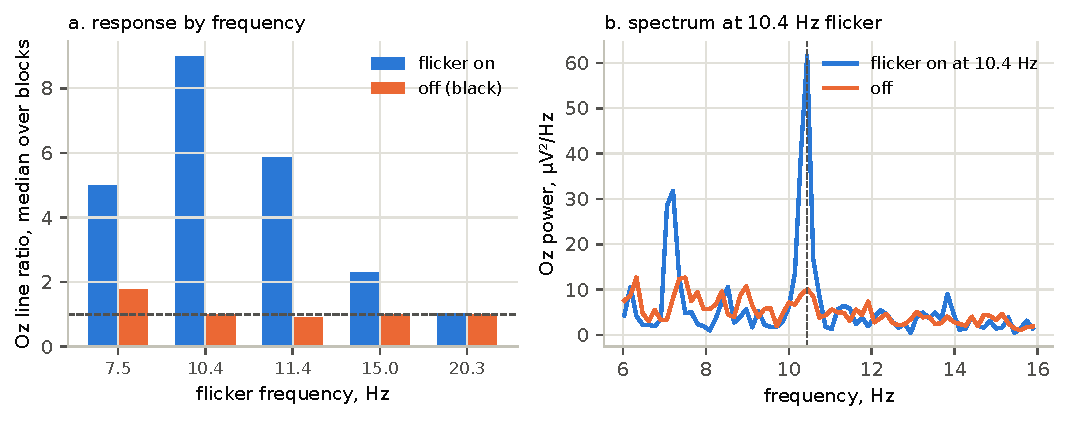
\includegraphics[width=\columnwidth]{response_curve}
\caption{The subject's response by frequency on the laptop (left) and the Oz spectrum at 10.4\,Hz flicker (right): a single-bin line with the alpha hump unchanged.}
\label{fig:sweep}
\end{figure}

\section{Results}

All results are from one subject, the first author, September to October 2026.

\textbf{Where the eye answers.} The first sweep (Fig.~\ref{fig:sweep}) put the response between 7.5 and 12\,Hz: Oz line ratios of 9.0 at 10.4\,Hz and 5.9 at 11.4\,Hz against 1.0 with the screen off, nothing at 20\,Hz. Mann's 15\,Hz sits on the weak side of this curve, so our sessions use 12\,Hz, the nearest frequency the display delivers exactly. A stock Muse without the cup showed no response. Measure the subject first.

\textbf{A legible word.} ``NO'' in a pixel font on 9 by 5 positions (Fig.~\ref{fig:no}): $r = 0.79$ after one pass, 0.88 after two, 0.91 after three, nulls at most 0.23, 43 of 45 positions right after the threshold, 18 minutes. A square 4.6 times larger reached 0.87 in two passes, so a larger square did not buy signal; a scalable font squeezed onto 48 positions was a blob before any brain was involved ($r = 0.41$ to 0.49 against nulls to 0.48).

\begin{figure*}[t]
\centering
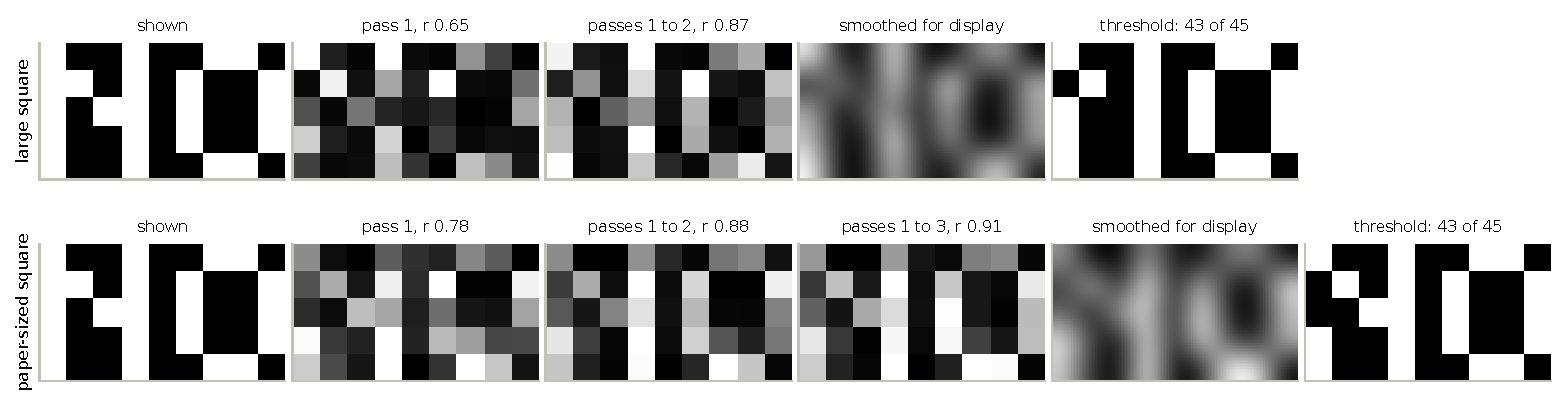
\includegraphics[width=0.92\textwidth]{no_word}
\caption{``NO'' read from the EEG in the Quest 3S, 12\,Hz, 8\,s per position, with a large square (top) and the paper-sized square (bottom): shown, after each pass, smoothed as in the 2019 paper, and thresholded. Both reach 43 of 45.}
\label{fig:no}
\end{figure*}

\textbf{Eight colours over three sittings.} Table~\ref{tab:colour} and Fig.~\ref{fig:colour9} and~\ref{fig:planes}. The first sitting read red 32, green 28 and blue 28 of 32, giving 24 of 32 cells in the right colour and the hue right on 19 of 24 coloured cells, $r = 0.79$ against nulls of 0.32. Two hours later, 20 of 32: green's second pass helped, blue's second pass was lost to the right ear electrode coming loose at minute 11. Two days later, 23 of 32, red perfect again, blue lost on the right half of the field with every electrode holding. One wrong cell in four on the chart is almost entirely blue's.

\begin{table}[t]
\caption{The eight-colour chart (8 by 4) over three sittings: cells right per plane, cells in the right colour, coloured cells with the right hue, and colour $r$ with the largest time-shifted null.}
\label{tab:colour}
\centering
\begin{tabular}{lcccccc}
\toprule
sitting & R & G & B & right & hue & $r$ (null) \\
\midrule
2026-10-10 17:57 & 32 & 28 & 28 & 24/32 & 19/24 & 0.79 (0.32) \\
2026-10-10 19:50 & 29 & 31 & 23 & 20/32 & 16/24 & 0.66 (0.32) \\
2026-10-12 10:40 & 32 & 31 & 23 & 23/32 & 16/24 & 0.75 (0.25) \\
\bottomrule
\end{tabular}
\end{table}

\begin{figure*}[t]
\centering
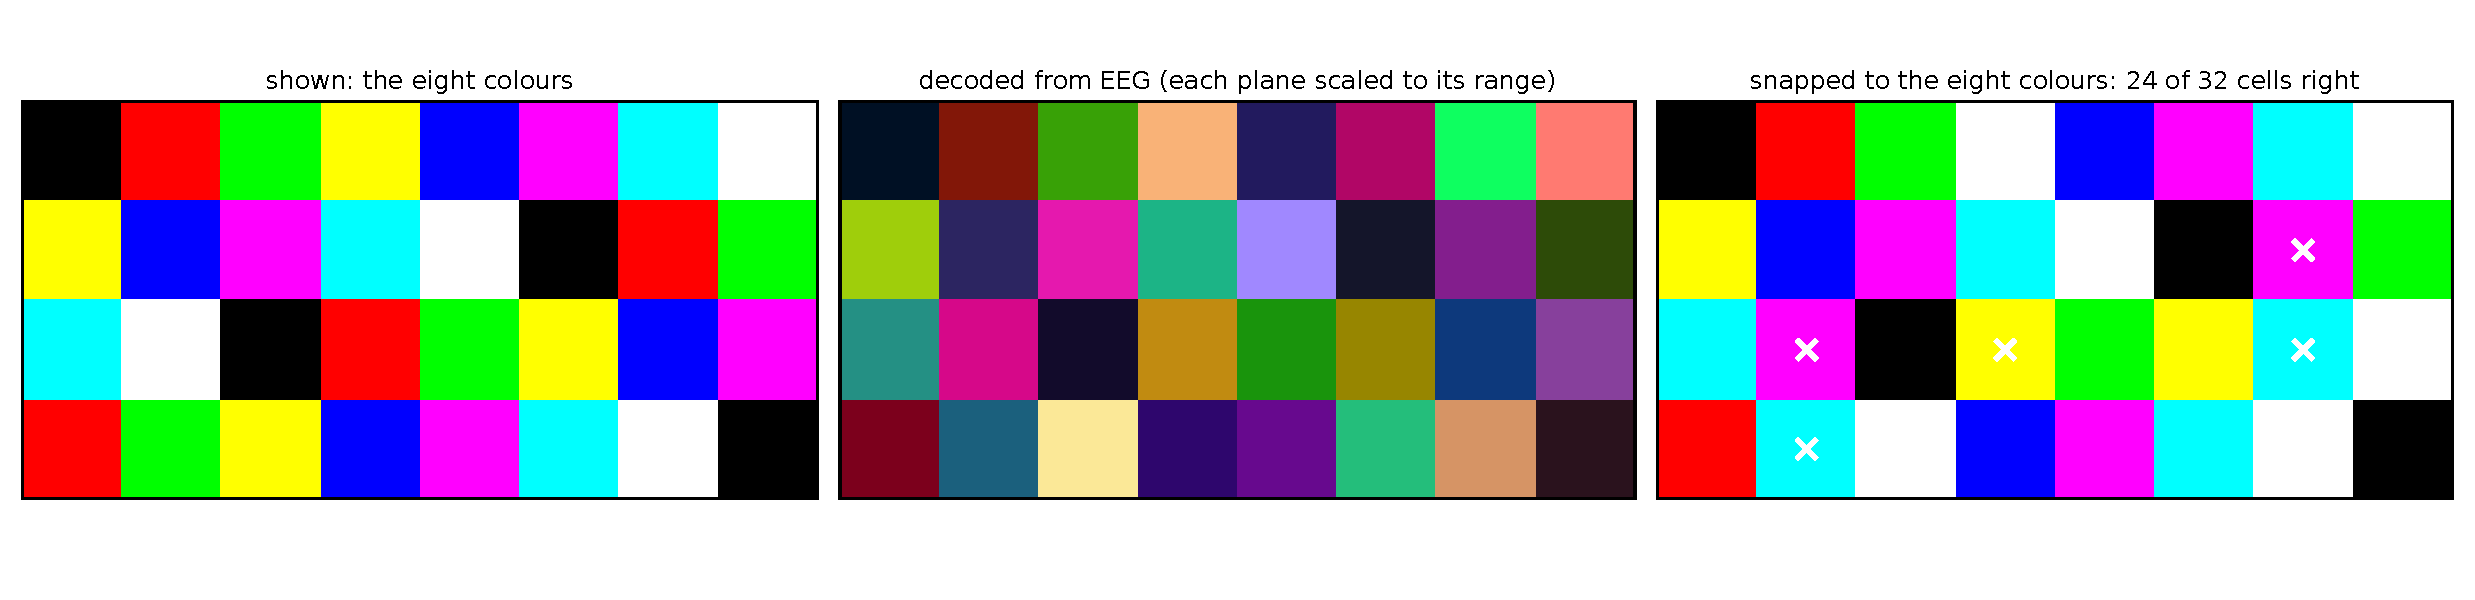
\includegraphics[width=0.92\textwidth]{colour_planes9}
\caption{Eight colours on the first colour sitting: shown, decoded with each plane scaled to its range, and snapped to the eight colours with wrong cells marked. 24 of 32.}
\label{fig:colour9}
\end{figure*}

\begin{figure}[t]
\centering
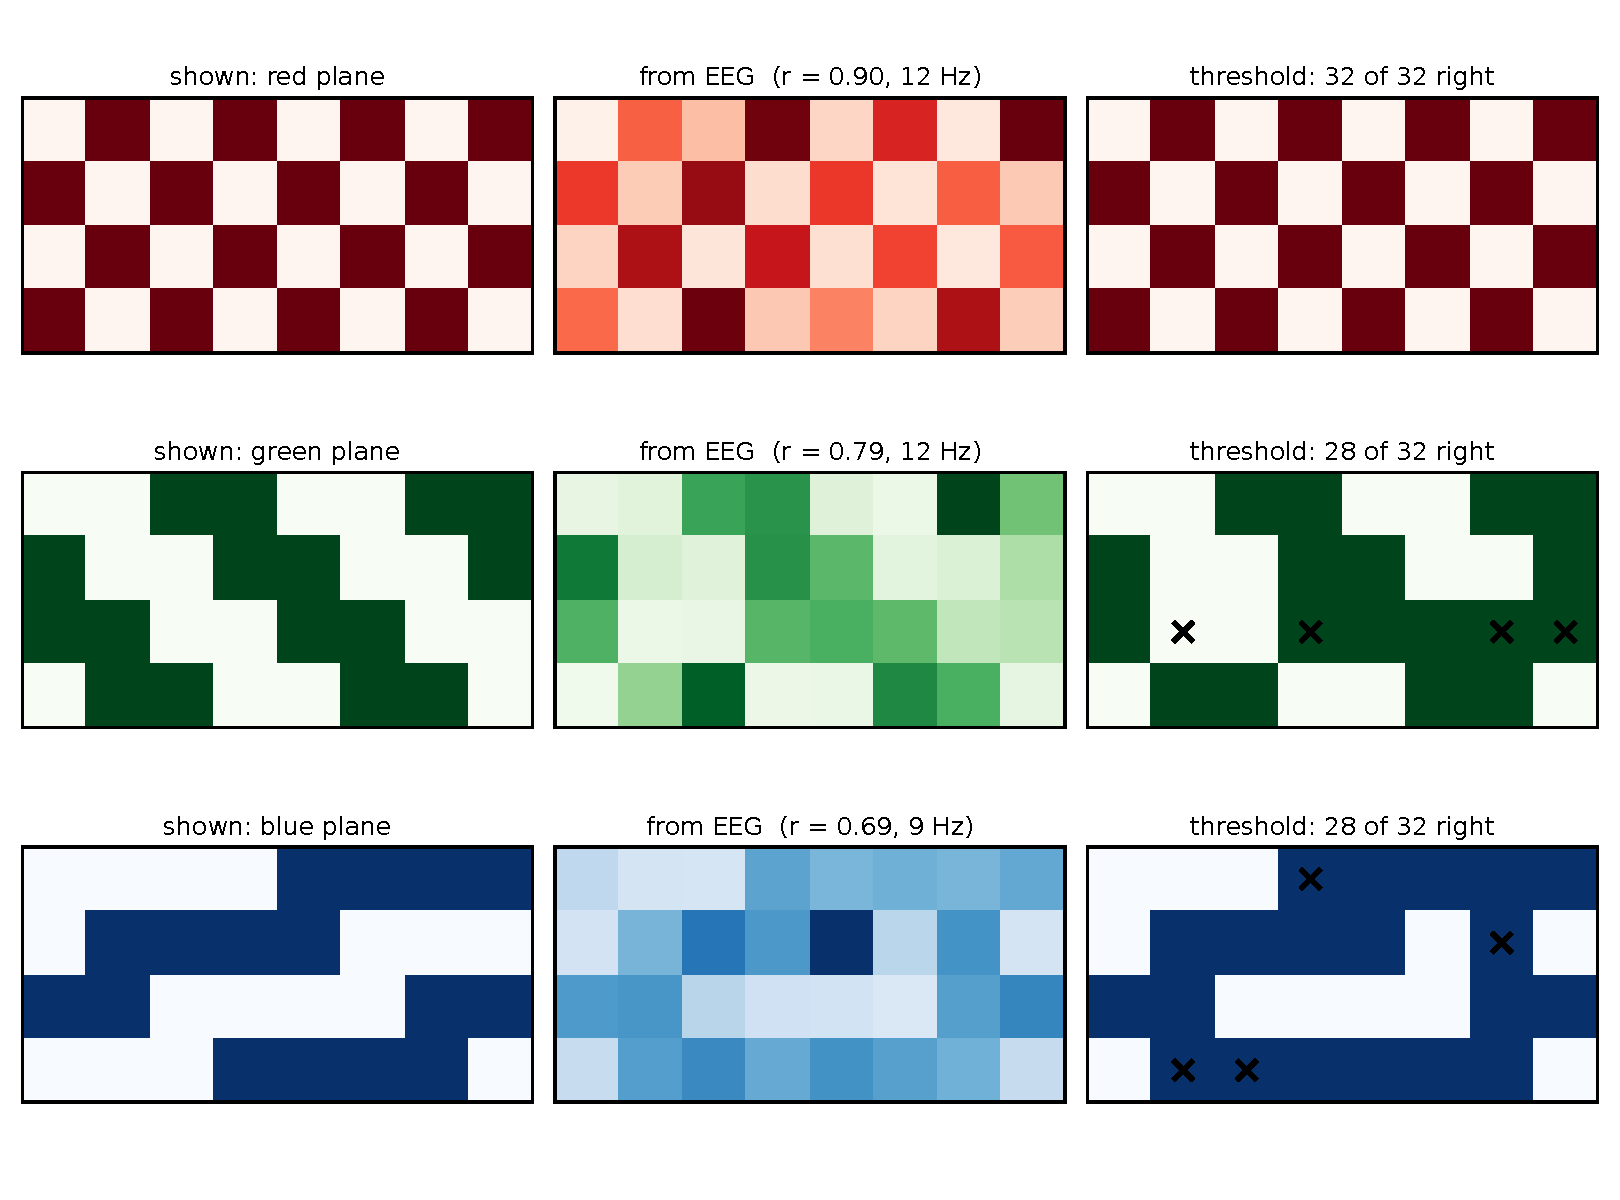
\includegraphics[width=0.78\columnwidth]{planes9_per_plane}
\caption{The same sitting plane by plane: shown, from the EEG, thresholded. Red 32, green 28, blue 28 of 32; blue at 9\,Hz with the patch doubled.}
\label{fig:planes}
\end{figure}

\textbf{A sealed acuity read-out.} A tumbling E and a ring that is closed (O) or missing its bottom (U) sit on a 12 by 7 grid; one of the eight combinations is drawn at random and sealed before the scan. A template correlation on the EEG picture names the orientation and the ring, then the seal is opened. On the first human run (Fig.~\ref{fig:acuity}) the picture reached $r = 0.89$, 80 of 84 cells, and the read-out said E up, ring U, with margins of 0.24 and 0.22 over the runners-up; the seal agreed. One trial at a one-in-eight chance is a demonstration, not an acuity measurement; a series over optotype sizes is the next step \cite{norcia1985sweep}.

\begin{figure*}[t]
\centering
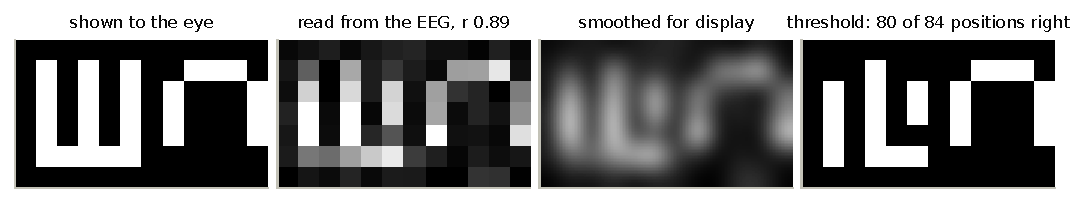
\includegraphics[width=0.92\textwidth]{acuity_vision1}
\caption{The sealed pair read from the EEG: shown, one value per position, smoothed, thresholded. The read-out named E up and ring U before the seal was opened; both right.}
\label{fig:acuity}
\end{figure*}

\textbf{Toward a real photograph.} The 2019 portrait went in thresholded to two tones and came back a silhouette. We prepare the same at our grid and add a forced choice: four portraits (Fig.~\ref{fig:gallery}) cut to 16 by 16 cells at four grey levels, the block-portrait size at which a face is recognisable \cite{harmon1973masking, harmon1973faces}; one is drawn and sealed, and the read-out names the person by correlation against all four. On the clean targets the choice is right 100\% of the time with a quarter of the cells flipped, chance one in four. A colour photograph does not survive the three planes (its colours sit mid-cube and flip), but a flat illustration in the eight corner colours does (Fig.~\ref{fig:gallery}, right). \todo{wedge result, first sealed photograph, officer scan}

\begin{figure}[t]
\centering
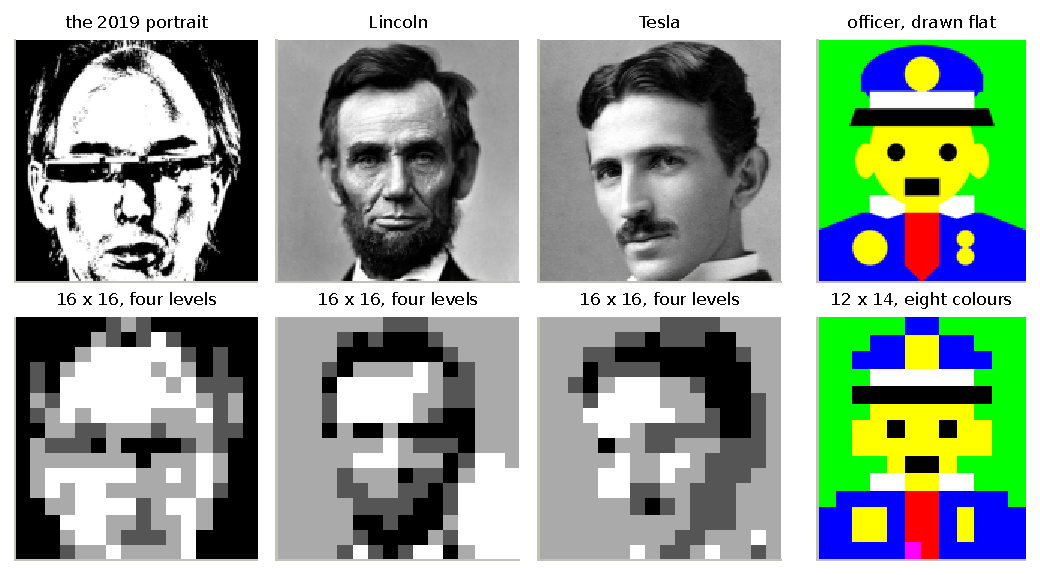
\includegraphics[width=\columnwidth]{gallery_16}
\caption{The photograph gallery: the crop the eye gets over its 16 by 16 four-level target, for Mann's 2019 portrait, Lincoln and Tesla (Einstein completes the set); right, the officer as a flat illustration and its 12 by 14 poster for the colour planes.}
\label{fig:gallery}
\end{figure}

\textbf{Eye strain from the same recording.} After two colour sittings in one evening the subject reported irritated eyes, a slight forehead ache and no drowsiness. On a Muse under a headset the blink is best seen through the Fpz reference on the far electrodes, as a shared deflection on TP9, TP10 and the cup. Counted so, the blink rate was 6.8 per minute in the first sitting and 12.1 in the second against 3 to 4 on a reference day, with amplitude and duration unchanged. Within a sitting (Fig.~\ref{fig:blink}) blinks nearly stop while a cell flickers and burst within a second of it going dark, 50 to 65 per minute in that second, a suppress-and-release pattern the reference day lacks \cite{stern1994blink, sheedy2003cvs}. Drowsiness markers were flat: no rise in frontal theta, no long blinks; an earlier report of rising alpha was the loose ear electrode and is retracted. The forehead ache is not in the EEG (frontalis 1.5 to 2.3\,$\mu$V rms); the headset's facial interface is the likelier cause. The SSVEP itself fell by half between the blue planes of the two sittings (Fig.~\ref{fig:fatigue}), and the cup's noise rose from minute 20 of the second, so part of what reads as fatigue is contact.

\begin{figure}[t]
\centering
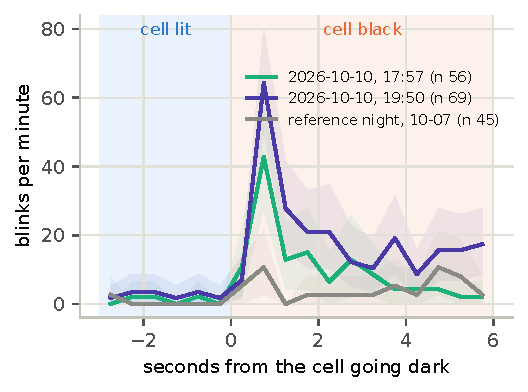
\includegraphics[width=0.9\columnwidth]{blink_release}
\caption{Blink release when the cell goes dark: blinks per minute in half-second bins around the moment a flickering cell turns black, two colour sittings against a reference day. Bands are 95\% block-bootstrap intervals.}
\label{fig:blink}
\end{figure}

\begin{figure}[t]
\centering
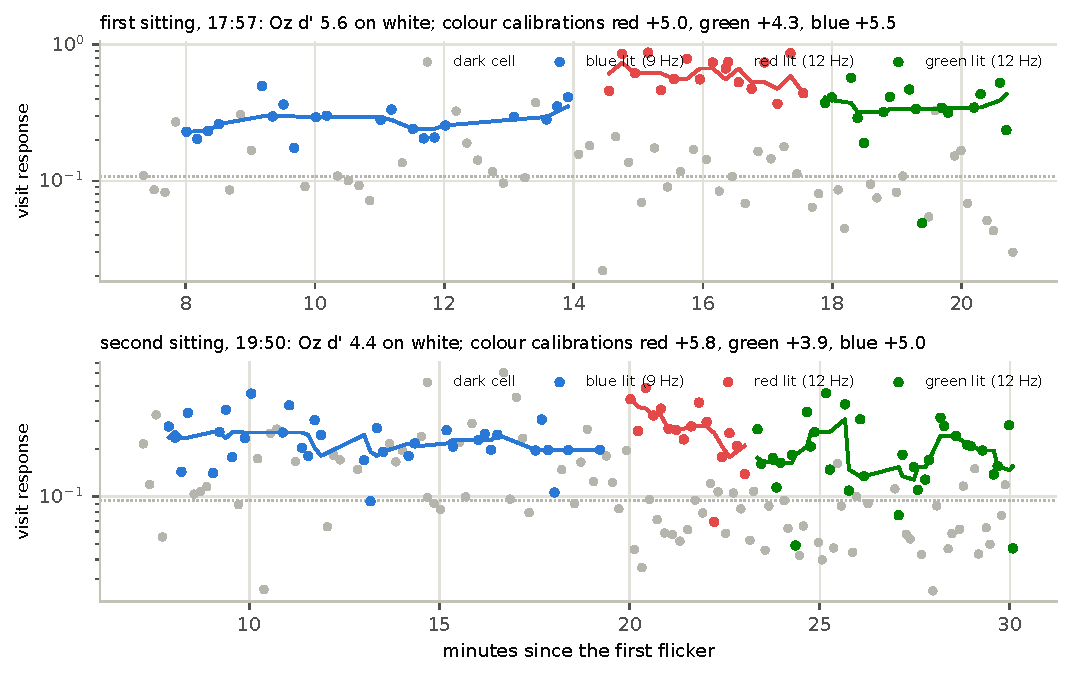
\includegraphics[width=0.9\columnwidth]{ssvep_fatigue_left}
\caption{The SSVEP of every lit cell through the two sittings of one evening (top the first, bottom the second), by plane. The blue response fell by half between them.}
\label{fig:fatigue}
\end{figure}

\section{Toward a Screening Tool for the Field}

What a community health worker would do with this decides the design. The metaveillography lineage says what the readings are: a visual field read from the brain, an acuity read from the brain, and an attention state read from how the field narrows and widens \cite{mann2019eye, garcia2020painting, garcia2021acuity}, all from hardware that costs less than a phone. Three readings come from one sitting under half an hour. A \emph{colour response profile}: the per-colour calibrations are three numbers before any scan (red, green, blue line statistics of +5.0, +4.3, +5.5 on the first sitting), the raw material of an objective colour-vision screen once the stimuli are isoluminant, which our smooth-flicker mode can display, and there is more than one subject. \rf{what a colour screen must report for a worker to act on it} An \emph{acuity read-out}: the sealed optotype, then a threshold series, giving acuity without a verbal response, as the sweep VEP does in a clinic \cite{norcia1985sweep}. An \emph{eye-strain reading and a prompt}: the blink pattern and rate are live from the same headband, and a ``rest your eyes'' message is the simplest just-in-time intervention \cite{nahum2018jitai}. \rf{prompt design and what to log around it}

\textbf{Limits.} One subject. One cell in four wrong on a 32-cell colour chart; a 96-cell picture is an hour. Blue is fragile, and 9\,Hz sits next to alpha. Contact is the largest practical risk: the cup's $\dprime$ ranged from 0.8 to 5.6 across days, and one loose electrode cost a plane. Flicker at 3 to 30\,Hz can provoke seizures in photosensitive epilepsy and the method must not be used with anyone with that history. The eye-strain result is one evening without a control. \rf{field constraints: time per subject, lighting, who holds the laptop} Next: two more subjects, the acuity series, the loose-channel guard, the sealed photograph, the prompt.

\section{Conclusion}

The eye as a camera works on a \$250 headband with one added cup and a \$300 headset: a legible word, eight colours over three sittings, and an optotype named from the EEG before its seal was opened, from a subject who only looked at a dot. The recording that gives the image also gives the eye strain. That is the start of a visual screener in the low-cost, objective, worker-operated tradition; the rest is subjects, stimuli that separate colour from brightness, and a prompt that closes the loop.

\section*{Acknowledgements}
\todo{MannLab Canada; Interaxon for the auxiliary-electrode documentation. Confirm wording.}

\bibliographystyle{IEEEtran}
\bibliography{refs}

\end{document}
